\chapter[Sprint 4 : Surveillance d'intégrité]{Sprint 4 : Une surveillance d'intégrité\\multicouche pour des entretiens fiables}
\begin{spacing}{1.2}
\minitoc
\thispagestyle{MyStyle}
\end{spacing}
\clearpage

\providecommand{\screenshot}[2]{%
  \IfFileExists{../screenshoot/#1}{%
    \includegraphics[width=0.9\textwidth,height=12cm,keepaspectratio]{../screenshoot/#1}%
  }{%
    \fbox{\parbox[c][4.5cm][c]{0.9\textwidth}{\centering\itshape
      Capture d'écran à insérer~: #2\\[4pt]
      \normalfont\small(fichier attendu~: \texttt{screenshoot/#1})}}%
  }%
}

\section{Introduction}

Le quatrième sprint consolide la salle d'entretien en y intégrant la surveillance d'intégrité et fiabilise l'ensemble des micro-services. Il met en place le détecteur de fraude à trois niveaux (MediaPipe côté client, vérification faciale InsightFace, détection d'objets YOLOv8n) ainsi que l'écran de vérification préalable à l'entretien.

\section{Objectifs du sprint}

L'objectif principal de ce sprint est défini comme suit~:

\begin{quote}
\itshape Garantir l'intégrité des entretiens à distance par une surveillance multicouche~: détecter en temps réel les comportements suspects (visages multiples, objets interdits, perte d'attention, usurpation d'identité) tout en préservant la confidentialité du candidat et en laissant la décision finale au recruteur.
\end{quote}

\subsection{Backlog du sprint}

Le tableau~\ref{tab:backlog-s4} présente le backlog du Sprint~4.

\begin{table}[H]
  \centering
  \footnotesize
  \renewcommand{\arraystretch}{1.3}
  \setlength{\tabcolsep}{5pt}
  \begin{tabularx}{\textwidth}{|>{\centering\arraybackslash}p{1.1cm}|>{\raggedright\arraybackslash}X|>{\centering\arraybackslash}p{1.8cm}|}
    \hline
    \rowcolor{blue!10}
    \textbf{ID} & \textbf{Récit utilisateur} & \textbf{Priorité} \\
    \hline
    S1 & En tant que recruteur, je veux être alerté si un autre visage ou une autre personne apparaît pendant l'entretien. & Haute \\
    \hline
    S2 & En tant que recruteur, je veux détecter la présence d'objets interdits (téléphone, écran, notes). & Haute \\
    \hline
    S3 & En tant que recruteur, je veux vérifier en continu que le candidat est bien la personne enrôlée. & Haute \\
    \hline
    S4 & En tant que candidat, je veux passer un contrôle préalable (caméra, microphone, identité) avant d'entrer en entretien. & Haute \\
    \hline
    S5 & En tant que recruteur, je veux consulter un rapport d'intégrité horodaté à l'issue de l'entretien. & Haute \\
    \hline
  \end{tabularx}
  \caption{Backlog du Sprint~4 : Surveillance d'intégrité.}
  \label{tab:backlog-s4}
\end{table}

\section{Concept de la surveillance d'intégrité}

Avec le passage au recrutement à distance, l'intégrité de l'entretien devient un enjeu à la fois technique et éthique. NextHire y répond par une surveillance \textit{multicouche}~: plutôt que de s'appuyer sur un unique indicateur, source de faux positifs bien documentés, la plateforme croise plusieurs signaux de détection, exécutés là où ils sont les plus pertinents.

Trois principes guident cette conception~: la \textbf{défense en profondeur} (plusieurs détecteurs indépendants), la \textbf{minimisation des données biométriques} (les trames transmises au serveur pour la vérification faciale et la détection d'objets sont traitées en mémoire et jamais persistées~; seuls les vecteurs d'\textit{embedding} qui en résultent sont conservés) et la \textbf{décision humaine}~: aucune violation ne disqualifie automatiquement un candidat~; toutes sont horodatées et remontées au recruteur, qui tranche.

\section{Conception détaillée et architecture}

\subsection{Architecture multicouche du détecteur}

Contrairement à une approche monolithique où l'ensemble de la détection s'exécuterait dans
un unique serveur, NextHire répartit la surveillance d'intégrité sur trois couches
complémentaires, ce qui réduit la charge réseau~: la première couche (MediaPipe) s'exécute
entièrement dans le navigateur et ne transmet aucune image, tandis que les deux couches
serveur (vérification faciale, détection d'objets) reçoivent des trames de la webcam mais
les traitent en mémoire sans jamais les persister :

\begin{itemize}
  \item \textbf{Analyse côté client (React).} Le composant \texttt{VisionMonitor} exécute
        directement dans le navigateur le modèle \textit{MediaPipe Face Landmarker}
        (bibliothèque \texttt{@mediapipe/tasks-vision}) à une cadence de 5~images/s. Il assure
        la détection du visage, le contrôle de présence, de centrage, de distance, de
        l'éclairage et de l'attention, sans transmettre la vidéo au serveur.
  \item \textbf{Service de vérification d'identité (Python / Flask).} Le service
        \texttt{face\_verification\_service} encapsule le modèle \textit{InsightFace}
        (\texttt{buffalo\_l}) via ONNXRuntime pour la confrontation d'identité 1:1.
  \item \textbf{Service de détection d'objets (Python / FastAPI).} Le service
        \texttt{yolo-service} encapsule le modèle \textit{YOLOv8n} pour la détection d'objets
        interdits dans le champ de la caméra.
\end{itemize}

Les événements produits par ces trois couches sont transmis au backend Node.js via
Socket.IO et REST, puis horodatés et enregistrés dans le document \texttt{CallRoom} de la
session. Par conception, ces détecteurs ne produisent que des constats objectifs (présence
d'objet, nombre de personnes, identité) : ils n'infèrent ni émotion, ni stress, ni
caractéristique personnelle, et le recruteur demeure le seul décideur final. La figure~\ref{fig:cheat-pipeline} synthétise ce pipeline de détection.

\begin{figure}[H]
  \centering
  \resizebox{0.88\textwidth}{!}{%
  \begin{tikzpicture}[
    font=\scriptsize,
    >=Stealth,
    src/.style={draw, rounded corners=3pt, fill=blue!12,
                minimum width=2.8cm, minimum height=0.60cm, align=center, font=\tiny\bfseries},
    evt/.style={draw=gray!45, rounded corners=2pt, fill=gray!7,
                minimum width=2.8cm, align=center, font=\tiny, text width=2.6cm, inner sep=2pt},
    agg/.style={draw, rounded corners=3pt, fill=orange!12,
                minimum width=11.0cm, minimum height=0.65cm, align=center, font=\tiny\bfseries},
    logb/.style={draw, rounded corners=3pt, fill=blue!8,
                 minimum width=11.0cm, minimum height=0.65cm, align=center, font=\tiny},
    rep/.style={draw, rounded corners=3pt, fill=green!10,
                minimum width=11.0cm, minimum height=0.65cm, align=center, font=\tiny},
    post/.style={draw, rounded corners=3pt, fill=purple!8,
                 minimum width=11.0cm, minimum height=0.65cm, align=center, font=\tiny},
  ]

  %% ── Source service boxes (top row) ──────────────────────────────────────
  \node[src] (S1) at (-5.0, 0.5)  {MediaPipe\\(client React)};
  \node[src] (S2) at (-1.7, 0.5)  {InsightFace\\Face Verify :8011};
  \node[src] (S3) at (1.7,  0.5)  {YOLOv8n\\YOLO Vision :8001};
  \node[src] (S4) at (5.0,  0.5)  {Navigateur\\(client React)};

  %% ── Event type boxes ────────────────────────────────────────────────────
  \node[evt, below=0.35cm of S1] (E1) {
    NO\_FACE\\MULTI\_FACE\\LOOK\_AWAY\\LIGHTING
  };
  \node[evt, below=0.35cm of S2] (E2) {
    Cosine similarity\\vs stored embedding\\(512-d InsightFace)
  };
  \node[evt, below=0.35cm of S3] (E3) {
    PHONE\_VISIBLE\\MULTI\_PEOPLE\\SCREEN\_DEVICE\\REFERENCE\_MAT
  };
  \node[evt, below=0.35cm of S4] (E4) {
    TAB\_SWITCH\\FULLSCREEN\_EXIT\\COPY\_PASTE
  };

  %% ── Aggregation layer ───────────────────────────────────────────────────
  \node[agg] (AGG)  at (0, -3.0) {Violation Aggregator : Serveur Node.js BFF};
  \node[logb](LOG)  at (0, -4.1) {visionMonitoring.events + integrityEvents (MongoDB)};
  \node[rep]  (REP) at (0, -5.1) {integrityReportService : risk\_level, score 0--100, recommandation};
  \node[post] (PST) at (0, -6.2) {Post-analyse LangGraph (analysis\_service :8090)};

  %% ── Fan-in arrows from event boxes to aggregator ────────────────────────
  \draw[->] (E1.south) -- (E1.south |- AGG.north);
  \draw[->] (E2.south) -- (E2.south |- AGG.north);
  \draw[->] (E3.south) -- (E3.south |- AGG.north);
  \draw[->] (E4.south) -- (E4.south |- AGG.north);

  %% ── Vertical pipeline arrows ────────────────────────────────────────────
  \draw[->] (AGG) -- (LOG);
  \draw[->] (LOG) -- (REP);
  \draw[->] (REP) -- (PST);

  \end{tikzpicture}%
  }%
  \caption{Architecture du pipeline de détection de fraude en temps réel de NextHire.}
  \label{fig:cheat-pipeline}
\end{figure}

\subsection{Surveillance d'intégrité en temps réel}

La figure~\ref{fig:seq-integrity} illustre le flux de surveillance d'intégrité qui s'exécute
en parallèle de chaque session d'entretien. Le système combine la détection d'objets (YOLO),
la vérification continue d'identité (Face Verify) et la surveillance des actions navigateur
pour détecter en temps réel tout comportement suspect.

\begin{sloppypar}
\begin{enumerate}
  \item \textbf{Activation.} À l'ouverture de la salle d'entretien, le backend vérifie que
        le profil facial du candidat est bien enregistré (embedding InsightFace) et notifie
        le client que la surveillance est active.

  \item \textbf{Boucle d'analyse vidéo.} Durant l'entretien, le client envoie des trames
        vidéo encodées en Base64 via Socket.IO. Le backend les transmet en parallèle au service
        YOLO Vision (détection de téléphone, document, écran, personnes multiples) et au
        service Face Verify (correspondance d'identité par similarité cosinus). En cas de
        violation détectée, l'événement est enregistré dans le document \texttt{CallRoom}
        avec son type, sa sévérité et l'identifiant de la question en cours.

  \item \textbf{Événements navigateur.} La page surveille les changements d'onglet, la
        sortie du plein écran et les tentatives de copier-coller, et les transmet immédiatement
        au backend. Ces événements sont enregistrés avec la sévérité \textit{critical}.

  \item \textbf{Rapport d'intégrité.} À la fin de la session, le backend agrège tous les
        événements, calcule un score de risque global et persiste le
        \texttt{integrityReport} (niveau de risque, synthèse, recommandation recruteur)
        dans MongoDB.
\end{enumerate}
\end{sloppypar}

\begin{figure}[H]
  \centering
  \resizebox{\textwidth}{!}{%
  \begin{tikzpicture}[
    font=\scriptsize,
    >={Stealth[length=2mm]},
    msg/.style={->, thin},
    ret/.style={->, thin, dashed},
    lbl/.style={font=\tiny, fill=white, inner sep=1pt, midway, above},
    lifeline/.style={dashed, thin, gray!70},
    phdr/.style={draw, fill=blue!12, rounded corners=2pt, align=center,
                 font=\scriptsize\bfseries, minimum height=0.65cm, minimum width=2.7cm},
  ]

  %% ── Participants ──────────────────────────────────────────────────────
  \node[phdr] at ( 0, 0) {React\\(Client)};
  \node[phdr] at ( 4, 0) {Node.js\\(:3001)};
  \node[phdr] at ( 9, 0) {YOLO Vision\\(:8001)};
  \node[phdr] at (14, 0) {Face Verify\\(:8011)};
  \node[phdr] at (19, 0) {MongoDB};

  %% ── Lifelines ─────────────────────────────────────────────────────────
  \draw[lifeline] ( 0,-0.38) -- ( 0,-15.0);
  \draw[lifeline] ( 4,-0.38) -- ( 4,-15.0);
  \draw[lifeline] ( 9,-0.38) -- ( 9,-15.0);
  \draw[lifeline] (14,-0.38) -- (14,-15.0);
  \draw[lifeline] (19,-0.38) -- (19,-15.0);

  %% ════════════════════════════════════════════════════════════════════════
  %% 1. Activation
  %% ════════════════════════════════════════════════════════════════════════
  \node[font=\tiny\bfseries, anchor=east] at (-0.3,-0.75) {1.};
  \draw[msg] ( 0,-0.75) -- node[lbl] {Socket.IO connect(roomId) + startMonitoring} (4,-0.75);
  \draw[msg] ( 4,-1.40) -- node[lbl] {POST /face-verify/start \{frames, liveness\}} (14,-1.40);
  \draw[ret] (14,-1.95) -- node[lbl] {\{status, similarity, threshold: 0.60\}} (4,-1.95);
  \draw[ret] ( 4,-2.50) -- node[lbl] {emit("monitoring-ready")} (0,-2.50);

  %% ════════════════════════════════════════════════════════════════════════
  %% 2. Loop — analyse vidéo
  %% ════════════════════════════════════════════════════════════════════════
  \node[font=\tiny\bfseries, anchor=east] at (-0.3,-2.95) {2.};
  \draw[draw=green!50!black, fill=green!5, rounded corners=3pt, dashed, thin]
    (-0.3,-2.95) rectangle (20.3,-9.70);
  \node[font=\tiny\bfseries, text=green!40!black, anchor=north west]
    at (-0.2,-3.00) {loop [chaque trame vidéo : environ 1 img / 1,5~s]};

  \draw[msg] ( 0,-3.65) -- node[lbl] {emit("video-frame", \{frame: base64, questionId\})} (4,-3.65);
  \draw[msg] ( 4,-4.25) -- node[lbl] {POST /detect-frame \{frame\}} (9,-4.25);
  \draw[ret] ( 9,-4.85) -- node[lbl] {\{objects: [...], persons: N\}} (4,-4.85);
  \draw[msg] ( 4,-5.45) -- node[lbl] {POST /face-verify/check \{frame\}} (14,-5.45);
  \draw[ret] (14,-6.05) -- node[lbl] {\{status, similarity\}} (4,-6.05);

  %% alt: violation détectée
  \draw[draw=red!50, fill=red!4, rounded corners=2pt, thin]
    (0.4,-6.55) rectangle (19.7,-9.30);
  \node[font=\tiny\bfseries, text=red!60!black, anchor=north west]
    at (0.5,-6.60) {alt [violation détectée : PHONE\_VISIBLE, MULTIPLE\_FACES, TAB\_SWITCH, ...]};
  \draw[msg] ( 4,-7.25) -- node[lbl] {enregistrer violation \{type, severity, evidence, questionId\}} (19,-7.25);
  \draw[ret] ( 4,-7.95) -- node[lbl] {emit("integrity-alert", \{type, severity\})} (0,-7.95);
  \draw[thin, gray!50] (0.4,-8.45) -- (19.7,-8.45);
  \node[font=\tiny, text=gray!55, anchor=west] at (0.5,-8.35) {else};
  \draw[ret] ( 4,-8.90) -- node[lbl] {emit("frame-ok")} (0,-8.90);

  %% ════════════════════════════════════════════════════════════════════════
  %% 3. Événements navigateur
  %% ════════════════════════════════════════════════════════════════════════
  \node[font=\tiny\bfseries, anchor=east] at (-0.3,-10.15) {3.};
  \draw[msg] ( 0,-10.15) -- node[lbl] {emit("browser-event", \{type: TAB\_SWITCH | FULLSCREEN\_EXIT\})} (4,-10.15);
  \draw[msg] ( 4,-10.80) -- node[lbl] {enregistrer événement \{type, severity: critical\}} (19,-10.80);
  \draw[ret] ( 4,-11.40) -- node[lbl] {emit("integrity-alert", \{type, severity: critical\})} (0,-11.40);

  %% ════════════════════════════════════════════════════════════════════════
  %% 4. Rapport d'intégrité
  %% ════════════════════════════════════════════════════════════════════════
  \node[font=\tiny\bfseries, anchor=east] at (-0.3,-12.00) {4.};
  \draw[->] (4,-12.00) -- ++(0.6,0) -- ++(0,-0.40) -- ++(-0.6,0);
  \node[font=\tiny, anchor=west] at (4.70,-12.20) {generateIntegrityReport(roomId)};
  \draw[msg] ( 4,-12.80) -- node[lbl] {sauvegarder integrityReport \{riskLevel, riskScore, keyFindings\}} (19,-12.80);
  \draw[ret] (19,-13.40) -- node[lbl] {200 OK} (4,-13.40);
  \draw[ret] ( 4,-13.90) -- node[lbl] {emit("integrity-report-ready", \{riskLevel, score\})} (0,-13.90);

  \end{tikzpicture}%
  }
  \caption{Diagramme de séquence : surveillance d'intégrité en temps réel.}
  \label{fig:seq-integrity}
\end{figure}

\section{Réalisation et interfaces utilisateur}

\subsection{Modules de détection}

\subsubsection{Détection du visage et de visages multiples}

Le \texttt{VisionMonitor} client s'appuie sur \textit{MediaPipe Face Landmarker} pour
localiser le visage du candidat sur chaque trame. L'absence prolongée de visage déclenche une
violation \texttt{NO\_FACE\_DETECTED}, tandis que la détection de plusieurs visages déclenche
\texttt{MULTIPLE\_FACES\_DETECTED}. En parallèle, la vérification d'identité continue est
confiée au service \textit{InsightFace} : pour chaque trame contrôlée, le service calcule
un \textit{embedding} facial normalisé de 512 dimensions et le compare, par similarité
cosinus, à l'\textit{embedding} de référence enregistré lors de l'inscription. Une similarité
inférieure au seuil de \texttt{0{,}60} signale une discordance d'identité.

\subsubsection{Suivi de l'attention et du cadrage}

À partir des points de repère faciaux fournis par \textit{MediaPipe Face Landmarker}, le
moniteur évalue en continu plusieurs indicateurs géométriques : le centrage du visage dans le
cadre (tolérances de \texttt{0{,}18} en horizontal et \texttt{0{,}20} en vertical), la
distance à la caméra estimée par le ratio surfacique du visage (plage acceptable de
\texttt{0{,}12} à \texttt{0{,}55}), la qualité de l'éclairage (luminance moyenne) et la
netteté de l'image. Une orientation du regard hors de l'écran maintenue au-delà du seuil
temporel déclenche une violation \texttt{LOOKING\_AWAY\_LONG}, et un visage mal cadré ou trop
éloigné produit respectivement \texttt{FACE\_NOT\_CENTERED} et \texttt{BAD\_FACE\_DISTANCE}.

\subsubsection{Détection d'objets}

Le service \texttt{yolo-service} charge le modèle pré-entraîné \textit{YOLOv8n} et restreint
les détections aux classes COCO pertinentes : téléphone (\texttt{cell phone}, 67), livre
(\texttt{book}, 73), ordinateur portable (\texttt{laptop}, 63), écran (\texttt{tv}, 62) et
personne (\texttt{person}, 0). Des seuils de confiance spécifiques par classe sont appliqués
(\texttt{0{,}30} pour le téléphone et le livre, \texttt{0{,}50} pour les écrans) afin de
limiter les faux positifs sur des trames webcam de 640~pixels. Chaque détection retenue est
convertie en violation typée : \texttt{PHONE\_VISIBLE}, \texttt{REFERENCE\_MATERIAL\_VISIBLE},
\texttt{SCREEN\_DEVICE\_VISIBLE}, \texttt{MULTIPLE\_PEOPLE} ou \texttt{NO\_PERSON\_VISIBLE}.

\subsection{Alerte d'intégrité en temps réel}

Lorsqu'une violation est détectée pendant l'entretien (par exemple un téléphone dans le champ de la caméra, la présence d'un second visage ou un changement d'onglet), une alerte est remontée en temps réel et l'événement correspondant est horodaté dans la session. La figure~\ref{fig:integrity-alert} en montre un exemple.

\begin{figure}[H]
  \centering
  \screenshot{integrity-alert.JPG}{Alerte d'intégrité affichée lors de la détection d'une violation}
  \caption{Exemple d'alerte d'intégrité en temps réel pendant l'entretien.}
  \label{fig:integrity-alert}
\end{figure}

\subsection{Production du rapport d'intégrité}

À la fin de la session, le backend Node.js agrège l'ensemble des violations enregistrées via
le service \texttt{integrityReportService}. Chaque type de violation contribue à un score de
risque pondéré : par exemple, la présence de plusieurs personnes ou de plusieurs visages
pèse 25~points, un téléphone ou un écran détecté 15~points, une absence du candidat 15~points,
et un changement d'onglet 10~points. Le score cumulé est plafonné à 100, puis traduit en un
niveau de risque (\textit{low} en deçà de 31, \textit{medium} de 31 à 65, \textit{high} à
partir de 66) accompagné d'une recommandation textuelle. Le rapport d'intégrité ainsi constitué est
persisté dans le document \texttt{CallRoom} et présenté au recruteur dans son tableau de bord
sous forme de chronologie d'événements et de cartes de synthèse (figure~\ref{fig:integrity-report}),
sans génération de fichier PDF externe.

\begin{figure}[H]
  \centering
  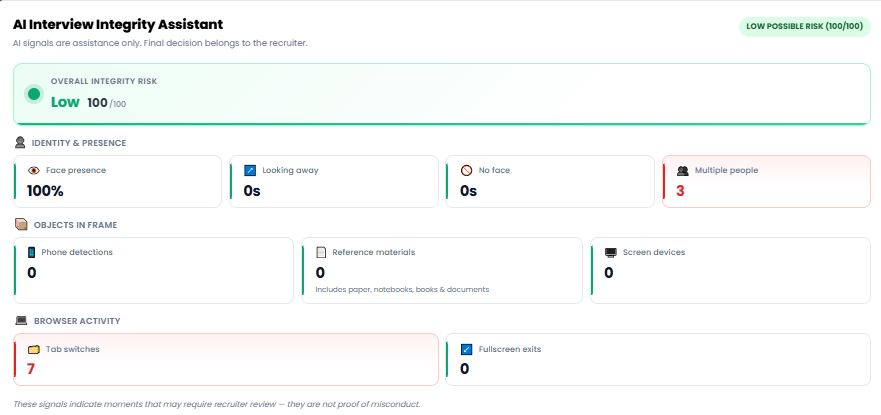
\includegraphics[width=0.9\textwidth,keepaspectratio]{../screenshoot/integrity.JPG}
  \caption{Exemple de rapport d'intégrité présenté au recruteur dans le tableau de bord NextHire.}
  \label{fig:integrity-report}
\end{figure}

\subsection{Écran de vérification pré-entretien}

Avant d'accéder à la salle d'entretien, le candidat passe par un écran de vérification
(composants \texttt{FaceVerification} et \texttt{VisionMonitor}). Celui-ci contrôle d'abord
les autorisations de la caméra et du microphone via l'API \textit{Permissions} du navigateur,
puis exécute un précontrôle en temps réel : présence et centrage du visage, qualité de
l'éclairage et unicité du visage dans le cadre. En parallèle, la vérification d'identité
faciale confronte l'image en direct à l'\textit{embedding} de référence du candidat
(InsightFace). Le candidat ne peut rejoindre l'entretien en direct que lorsque l'ensemble de
ces contrôles est validé (figure~\ref{fig:pre-interview}).

\begin{figure}[H]
  \centering
  \screenshot{pre-interview-verification.JPG}{Vérification caméra, micro et identité faciale}
  \caption{Écran de vérification pré-entretien.}
  \label{fig:pre-interview}
\end{figure}

\subsection{Vérification faciale \textit{fail-closed}}

Avant chaque entretien, un module de vérification d'identité compare l'image capturée en temps
réel par la webcam à la photo de profil enregistrée lors de l'enrôlement. La comparaison repose
sur un vecteur d'embedding de 512 dimensions calculé par InsightFace (modèle \texttt{buffalo\_l})
et une similarité cosinus. Le comportement est \textit{fail-closed} : toute condition anormale
bloque l'accès à la salle d'entretien plutôt que de le laisser passer.

\begin{itemize}
  \item \textbf{Service indisponible.} Si le micro-service de vérification faciale ne répond
        pas, la décision de démarrage est refusée (\texttt{status: 'failed',
        reason: 'face\_verification\_disabled'}).
  \item \textbf{Candidat non enrôlé.} Si aucun profil facial n'a été préalablement enregistré
        pour le candidat, l'accès est bloqué et un événement d'audit
        \texttt{NOT\_ENROLLED} est enregistré.
  \item \textbf{Similarité insuffisante.} Si la similarité cosinus entre les deux embeddings
        est inférieure au seuil $\tau = 0{,}60$, la vérification échoue et l'événement est journalisé
        avec les métadonnées d'audit (nombre de trames valides, score moyen).
\end{itemize}

La confidentialité est préservée par conception : les trames webcam transmises au serveur
pour la vérification ne sont jamais persistées et sont traitées en mémoire par le service
Python le temps du calcul de l'\textit{embedding}. Seul ce vecteur de 512 dimensions est
conservé, ce qui limite l'exposition des données biométriques au strict nécessaire. La figure~\ref{fig:face-verify-failed} illustre le cas où l'accès est refusé faute de correspondance d'identité.

\begin{figure}[H]
  \centering
  \screenshot{face-verify-failed.JPG}{Accès refusé : l'identité ne correspond pas au profil enrôlé}
  \caption{Comportement \textit{fail-closed} : accès à la salle refusé en cas de discordance d'identité.}
  \label{fig:face-verify-failed}
\end{figure}

\section{Tests}

\subsection{Test de la décision de vérification faciale}

Le module décisionnel de la vérification faciale est couvert par un test en
\texttt{node:assert} (\texttt{faceVerifyDecision.test.js}) regroupant 12~assertions. Celles-ci
vérifient le comportement \textit{fail-closed} de la décision de démarrage d'entretien :
la projection de sélection des candidats n'expose jamais l'\textit{embedding} facial parent,
une correspondance stricte n'est validée que lorsque le nombre minimal de trames concordantes
est atteint, et toute configuration ambiguë conduit à un refus plutôt qu'à une autorisation.

\section{Conclusion}

Ce sprint a fiabilisé la salle d'entretien en la dotant d'une surveillance d'intégrité multicouche et d'une vérification d'identité \textit{fail-closed}, sans jamais exposer les images brutes du candidat. Le sprint suivant complète la plateforme par l'aide à la décision (rapports pondérés, comparaison des candidats), le tableau de bord administrateur et la phase de finalisation.
